\documentclass[a4j]{jarticle}
%%  packages
\usepackage{amsmath,amssymb,ascmac}
\usepackage{bm}
\usepackage[dvipdfmx]{graphicx}
\usepackage{listings}
\usepackage[english]{babel}
\lstset{
 	%枠外に行った時の自動改行
 	breaklines = true,
 	%標準の書体
        basicstyle=\ttfamily\footnotesize,
        commentstyle=\footnotesize\bfseries,
        keywordstyle=\footnotesize\bfseries,
 	%枠 "t"は上に線を記載, "T"は上に二重線を記載
	%他オプション:leftline,topline,bottomline,lines,single,shadowbox
 	frame = single,
 	%frameまでの間隔(行番号とプログラムの間)
 	framesep = 5pt,
 	%行番号の位置
 	numbers = left,
	%行番号の間隔
 	stepnumber = 1,
	%タブの大きさ
 	tabsize = 4,
 	%キャプションの場所("tb"ならば上下両方に記載)
 	captionpos = t
}
%% title configuration
\title{Template}
\author{John Smith}
\date{\today}

\let \ds \displaystyle

%% headings
\pagestyle{myheadings}
\markboth{}{This is Sample.}


%% document
\begin{document}
%%  begin title page
\maketitle
\pagebreak


\newcommand{\idiff}[3]{
  \frac{d^{#1} #2}{d #3^{#1}}
}
\newcommand{\diff}[3]{
  \frac{\mathrm{d}^{#1} #2}{\mathrm{d} #3^{#1}}
}
\newcommand{\pdiff}[3]{
  \frac{\partial^{#1} #2}{\partial #3^{#1}}
}

%% begin contents


$$ A \subset B \Leftrightarrow \forall x ( x \in A \Rightarrow x \in B) $$

$\displaystyle  e^x = \sum_{i=0}^\infty \frac{x^i}{i!}$  $ \Rightarrow \idiff{n}{}{x} e^x = e^x$

$\ds \pdiff{}{}{\bm{x}}\langle \bm{a},\bm{x} \rangle =\frac{\partial}{\partial \bm{x}} \left( \bm{a}^\top \bm{x}\right)= \frac{\partial}{\partial \bm{x}} \left( \bm{x}^\top \bm{a}\right) = \bm{a}$

\begin{lstlisting}[language=C]
#include <stdio.h>
#include <stdlib.h>
#include <time.h>

void handle_error (int retval){
     printf("[ERROR] error"); // handling
     exit(1);
}
\end{lstlisting}
\begin{lstlisting}[language=Python]
import numpy as np
N = 10
a = np.arrange(0,N)
for i in range(N):
    print(a[i])
\end{lstlisting}
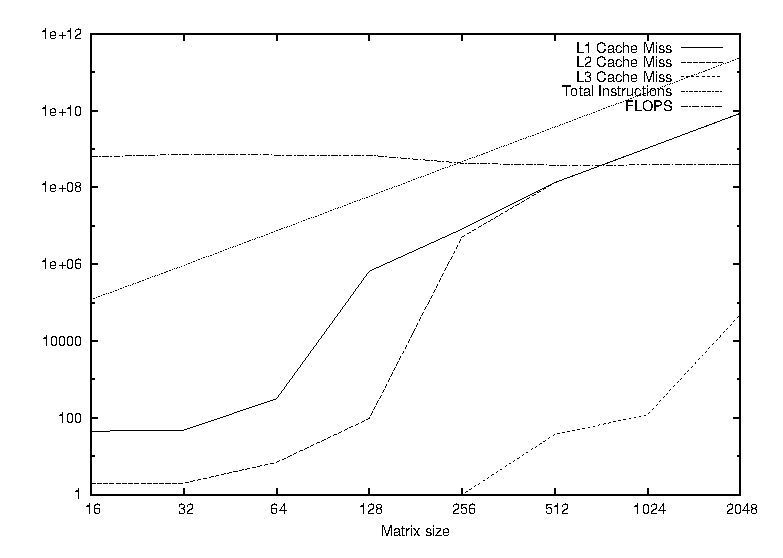
\includegraphics[width=10cm]{template.eps}
\pagebreak



\end{document}


